\documentclass[a4paper]{article}

\input{style/ch_xelatex.tex}
\input{style/scala.tex}

%代码段设置
\lstset{numbers=left,
basicstyle=\tiny,
numberstyle=\tiny,
keywordstyle=\color{blue!70},
commentstyle=\color{red!50!green!50!blue!50},
frame=single, rulesepcolor=\color{red!20!green!20!blue!20},
escapeinside=``
}

\graphicspath{ {images/} }
\usepackage{ctex}
\usepackage{graphicx}
\usepackage{color,framed}%文本框
\usepackage{listings}
\usepackage{caption}
\usepackage{amssymb}
\usepackage{enumerate}
\usepackage{xcolor}
\usepackage{bm} 
\usepackage{lastpage}%获得总页数
\usepackage{fancyhdr}
\usepackage{tabularx}  
\usepackage{geometry}
\usepackage{minted}
\usepackage{graphics}
\usepackage{subfigure}
\usepackage{float}
\usepackage{pdfpages}
\usepackage{pgfplots}
\pgfplotsset{width=10cm,compat=1.9}
\usepackage{multirow}
\usepackage{footnote}
\usepackage{booktabs}

%-----------------------伪代码------------------
\usepackage{algorithm}  
\usepackage{algorithmicx}  
\usepackage{algpseudocode}  
\floatname{algorithm}{Algorithm}  
\renewcommand{\algorithmicrequire}{\textbf{Input:}}  
\renewcommand{\algorithmicensure}{\textbf{Output:}} 
\usepackage{lipsum}  
\makeatletter
\newenvironment{breakablealgorithm}
  {% \begin{breakablealgorithm}
  \begin{center}
     \refstepcounter{algorithm}% New algorithm
     \hrule height.8pt depth0pt \kern2pt% \@fs@pre for \@fs@ruled
     \renewcommand{\caption}[2][\relax]{% Make a new \caption
      {\raggedright\textbf{\ALG@name~\thealgorithm} ##2\par}%
      \ifx\relax##1\relax % #1 is \relax
         \addcontentsline{loa}{algorithm}{\protect\numberline{\thealgorithm}##2}%
      \else % #1 is not \relax
         \addcontentsline{loa}{algorithm}{\protect\numberline{\thealgorithm}##1}%
      \fi
      \kern2pt\hrule\kern2pt
     }
  }{% \end{breakablealgorithm}
     \kern2pt\hrule\relax% \@fs@post for \@fs@ruled
  \end{center}
  }
\makeatother
%------------------------代码-------------------
\usepackage{xcolor} 
\usepackage{listings} 
\lstset{ 
breaklines,%自动换行
basicstyle=\small,
escapeinside=``,
keywordstyle=\color{ blue!70} \bfseries,
commentstyle=\color{red!50!green!50!blue!50},% 
stringstyle=\ttfamily,% 
extendedchars=false,% 
linewidth=\textwidth,% 
numbers=left,% 
numberstyle=\tiny \color{blue!50},% 
frame=trbl% 
rulesepcolor= \color{ red!20!green!20!blue!20} 
}

%-------------------------页面边距--------------
\geometry{a4paper,left=2.3cm,right=2.3cm,top=2.7cm,bottom=2.7cm}
%-------------------------页眉页脚--------------
\usepackage{fancyhdr}
\pagestyle{fancy}
\lhead{\kaishu \leftmark}
% \chead{}
\rhead{\kaishu 并行程序设计实验报告}%加粗\bfseries 
\lfoot{}
\cfoot{\thepage}
\rfoot{}
\renewcommand{\headrulewidth}{0.1pt}  
\renewcommand{\footrulewidth}{0pt}%去掉横线
\newcommand{\HRule}{\rule{\linewidth}{0.5mm}}%标题横线
\newcommand{\HRulegrossa}{\rule{\linewidth}{1.2mm}}
\setlength{\textfloatsep}{10mm}%设置图片的前后间距
%--------------------文档内容--------------------

\begin{document}
\renewcommand{\contentsname}{目\ 录}
\renewcommand{\appendixname}{附录}
\renewcommand{\appendixpagename}{附录}
\renewcommand{\refname}{参考文献} 
\renewcommand{\figurename}{图}
\renewcommand{\tablename}{表}
\renewcommand{\today}{\number\year 年 \number\month 月 \number\day 日}

%-------------------------封面----------------
\begin{titlepage}
    \begin{center}
    
\includegraphics[width=0.8\textwidth]{NKU.png}\\[1cm]
    \vspace{20mm}
		\textbf{\huge\textbf{\kaishu{计算机学院}}}\\[0.5cm]
		\textbf{\huge{\kaishu{并行体系结构调研}}}\\[2.3cm]
		\textbf{\Huge\textbf{\kaishu{我国超算发展历史与并行体系结构}}}

		\vspace{\fill}
    
    % \textbf{\Large \textbf{并行程序设计期末实验报告}}\\[0.8cm]
    % \HRule \\[0.9cm]
    % \HRule \\[2.0cm]
    \centering
    \textsc{\LARGE \kaishu{姓名\ :\ 王一诺}}\\[0.5cm]
    \textsc{\LARGE \kaishu{学号\ :\ 2312331}}\\[0.5cm]
    \textsc{\LARGE \kaishu{专业\ :\ 计算机科学与技术}}\\[0.5cm]
    
    \vfill
    {\Large \today}
    \end{center}
\end{titlepage}

\renewcommand {\thefigure}{\thesection{}.\arabic{figure}}%图片按章标号
\renewcommand{\figurename}{图}
\renewcommand{\contentsname}{目录}  
\cfoot{\thepage\ of \pageref{LastPage}}%当前页 of 总页数


% 生成目录
\clearpage
\tableofcontents
\newpage

%-------------------------引言----------------------------------
\section{引言}
超级计算机作为国家科技实力的战略制高点，既是前沿科学研究的“加速器”，也是大国科技博弈的“角力场”。从核聚变模拟到基因测序，从气候预测到人工智能训练，超算的算力水平直接决定了人类探索未知边界的深度与广度。自20世纪80年代以来，中国超算从“玻璃房”时代的屈辱起步，历经四十年筚路蓝缕，实现了从“亿次”到“百亿亿次”的算力跃迁，更以“神威·太湖之光”“天河”系列等里程碑式成果，在全球超算版图上刻下鲜明的中国坐标。

这一历程不仅关乎技术突破，更折射出国家意志与时代需求的共振。当西方国家以“玻璃房”监控限制中国使用进口超算时，银河一号的诞生宣告了自主研制的决心；当美国通过芯片禁运试图遏制天河二号的升级时，神威众核处理器的横空出世证明了国产替代的可行性。中国超算的崛起，本质上是一场“技术突围战”——既要突破物理层面的算力极限，更要打破制度性封锁与生态壁垒。

本报告立足历史纵深与国际视野，通过梳理中国超算的技术演进、剖析代表性超算并行体系架构、对比海外最新进展，试图揭示我国超算发展的优势与差距，展望未来方向。

%-------------------------我国超算发展历史----------------------------------
\section{我国超算发展历史}
中国超级计算机的技术演进是一部从模仿追赶到自主创新的历史，其核心路径始终围绕“自主可控”与“算力突破”两大主线展开。早期的技术路线受限于国际封锁与基础薄弱，但通过战略规划与科研攻坚，中国逐步构建起多元化的并行计算架构体系，并在关键领域实现跨越式突破。

\subsection{向量处理器时代（1970年代末-1990年代初）}
中国超算的起点以向量处理器架构为核心标志，其背景源于国防与科研领域对高性能计算的迫切需求。1978年，中央军委批准由国防科技大学承担亿次机研制任务，并于1983年推出首台自主超算“银河一号”。该机型采用向量处理器技术，通过单指令流多数据流（SIMD）并行模式优化科学计算，运算速度达1亿次/秒，主要用于核武器模拟、气象预测等领域。\cite{1}

尽管其性能仅为同期国际水平的十分之一，但标志着中国成为继美、日之后第三个具备超算研制能力的国家，打破了西方技术封锁的“玻璃房”屈辱历史。然而，向量架构的局限性在于编程复杂且扩展性差，难以满足通用计算需求，这一阶段更多是解决“有无问题”，为后续技术突破奠定基础。

\subsection{并行架构突破（1990年代-2000年代初）}
这一阶段的核心特征是从单一向量处理器向并行计算架构转型，突破技术封锁并提升计算效率。1992年研制成功的银河二号是中国首台十亿次级（1 GFLOPS）巨型计算机，其设计标志着中国超算从早期向量处理器（如银河一号）转向更复杂的并行计算架构。该机型采用多协议体系、多机种协同的并行网络系统，实现了多任务并行处理能力的显著提升。其自主研发的高速计算机网络系统被誉为“国内领先，达到80年代末国际先进水平”，为中国后续超算的分布式并行架构奠定了基础。

随着改革开放的深入、经济与科技的发展，中国超算转向对称多处理（SMP）架构，开启了共享内存并行计算的新阶段。1993年，国家智能计算机研究开发中心团队在硅谷完成“曙光一号”研发，采用Motorola M88100处理器，峰值性能6.4亿次/秒，并搭载国产SNIX操作系统。其SMP架构通过多核共享内存提升并行效率，但节点扩展性受限于内存带宽。曙光一号的诞生不仅迫使西方解除对华超算禁运，更推动了中国从模仿到自主创新的转型。此后，曙光系列持续迭代，1995年的曙光1000峰值速度达25亿次/秒，逐步构建起国产并行计算生态。

曙光4000A是中国首台峰值算力突破每秒10万亿次浮点运算（10 TFlops）的超级计算机，在2004年全球TOP500排行榜中位列第十，使中国成为继美国、日本之后第三个具备10万亿次超算研发能力的国家。其核心架构基于大规模机群系统（Cluster），整合了2000多颗64位AMD Opteron处理器，采用自主研发的机群操作系统和高速互连技术，实现了从科研专用设备向商业化高性能计算机的转型。

\subsection{异构计算崛起（2000年代-2010年代）}
21世纪初，中国超算引入CPU+加速器异构架构，算力密度显著提升。2009年，国防科技大学研发的“天河一号”以每秒4700万亿次算力登顶全球超算榜首，其采用Intel Xeon CPU与NVIDIA Tesla GPU混合架构，通过自主研发的TH-Express高速互连网络降低通信延迟。\cite{2}
2013年，“天河二号”虽以54.9千万亿次算力蝉联世界第一，但依赖进口Xeon Phi协处理器的问题仍制约其可持续发展。

\subsection{自主众核架构（2010年代末-2020年代初）}
为解决“卡脖子”问题，中国转向自主众核处理器设计，实现全链条国产化。2016年，“神威·太湖之光”采用申威26010众核处理器，单芯片集成260核心（4主核+256从核），峰值算力12.5亿亿次/秒，能效比达8.2GFlops/W。\cite{3}
其架构通过主从核分层管理与片上网络（NoC）优化通信效率，适用于高精度科学计算。该机型连续四年蝉联全球超算榜首，并在气候模拟、量子化学等领域获“戈登·贝尔奖”，验证了国产架构的应用价值。

\subsection{E级超算与混合架构（2020年代至今）}
当前，中国超算迈入百亿亿次（E级）时代，技术路线聚焦光互连、存算一体与AI融合。神威E级原型机采用光互连技术将节点间延迟降至微秒级，支持百万级核心扩展；天河三号则探索近内存计算架构，适配AI训练等高吞吐任务。尽管中国率先完成E级超算技术验证，但能效比（如神威93.01 TFlops/W[23年6月榜单]）仍显著落后于美国Frontier（1194 TFlops/W[23年6月榜单]），芯片制程依赖中芯国际14nm工艺的问题也亟待突破。

\section{代表性超算并行体系结构剖析}
\subsection{天河二号}
天河二号的并行架构以“异构融合+高速互连”为特色，代表了早期中国超算在进口芯片依赖下的技术突破。其异构体系整合了32,000颗Intel Xeon Ivy Bridge CPU与48,000个Xeon Phi协处理器，通过自主研发的TH-Express 2高速互连网络实现节点间低延迟（85微秒）通信，带宽达2.56 Tbps。每个计算节点采用“CPU+APU”双板设计，CPU板承载通用计算任务，APU板集成多个Xeon Phi协处理器，通过PCI-E2.0接口实现混合计算。\cite{4}

尽管依赖进口芯片，但其创新不容小看——异构任务调度框架与能效优化。系统通过动态负载均衡技术，将能效比提升至每瓦1.935 GFlops，连续六次登顶TOP500榜单。天河二号的应用创新同样显著，例如支撑宇宙中微子模拟（3万亿粒子规模）与埃博拉病毒药物筛选，验证了异构架构在科学工程计算中的潜力。

\subsection{神威·太湖之光}
神威·太湖之光的并行体系结构以“众核异构+片上网络”为核心，首次实现了全自主可控的超大规模并行计算。其核心处理器申威26010采用片上融合的异构众核设计，单芯片集成260个计算核心（4个主核+256个从核），主核负责任务调度与通信管理，从核专注于计算密集型任务，并通过片上网络（NoC）实现低延迟通信，显著降低数据搬运能耗。该架构突破了传统CPU+加速卡的分立式设计瓶颈，将运算控制核心与运算核心集成于单一芯片，避免了PCI-E接口的带宽限制，单芯片峰值性能达每秒3万亿次浮点运算。\cite{3}

如图\ref{fig:shenwei}所示
\begin{figure}[H]
	\centering
	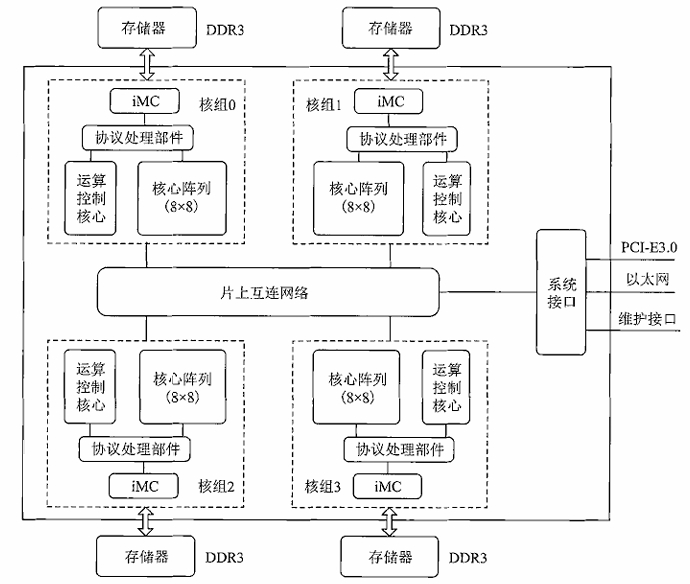
\includegraphics[scale=0.3]{申威26010.png}
	\caption{Caption}
	\label{fig:shenwei}
\end{figure}

系统层面，神威·太湖之光采用高密度超节点架构，整机由40960块申威处理器组成，支持千万核级并行规模，通过分层容错机制和自适应调度技术，确保大规模计算的稳定性与效率。

其创新性体现在两方面：一是首次实现全自主芯片与软件生态（如神威睿思操作系统），规避了技术封锁风险；二是通过低标度算法优化，成功支撑了数万原子级第一性原理计算等前沿科学任务，推动中国超算应用登上国际舞台。

\subsection{曙光E级原型机}
硬件层面，曙光E级采用混合存储结构，结合多级缓存优化数据访问效率，适配高吞吐任务（如深度学习训练）；软件层面，其支持混合精度计算（FP16/FP32），并通过跨平台调度系统整合区域算力资源（如“京数津算”模式），实现算力动态调配。

曙光E级原型机共有512个结点,102４颗Hygon处理器和512块DCU 加 速 卡。各结点之间使用200Gbps的高速网络，采用6D-Torus 的方式实现高维互连。

每个结点有2颗 H ygon 7185 处理器和1块DCU加速卡，256 GB的 DDR４ 内存，2４0 GB 的M.2 SSD 硬盘。具体架构如图 \ref{fig:shuguang} 所示。\cite{5}
\begin{figure}[H]
	\centering
	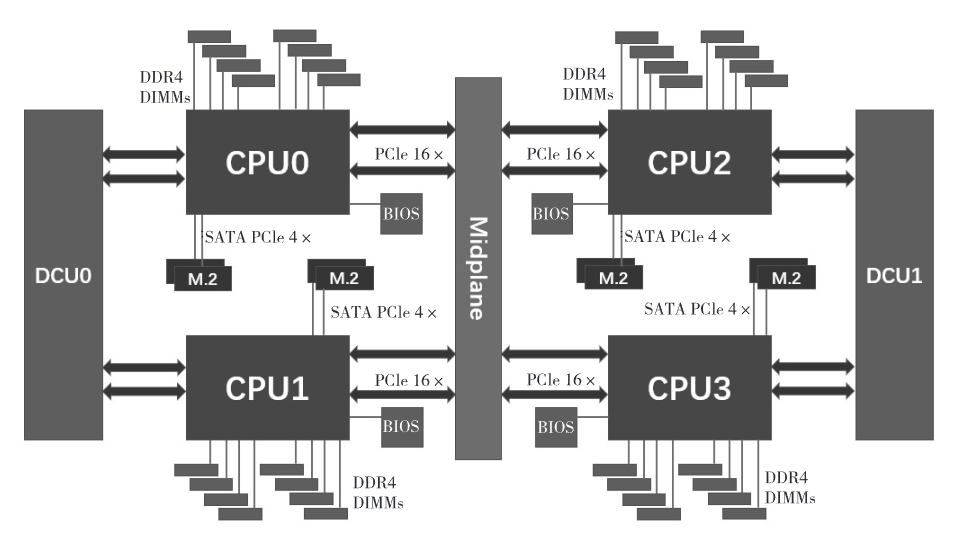
\includegraphics[scale=0.3]{曙光E级.png}
	\caption{Caption}
	\label{fig:shuguang}
\end{figure}

\subsection{神威E级超算}
神威E级原型机由1024个申威26010+众核处理器(简称SW26010+)组成，每个处理器包含4个运算控制核心和256个运算核心．2个处理器通过PCIe3．o连接到同一片网络接口芯片，构成一个运算节点，每个运算节点峰值运算能力6．12 TFlops．512个运算节点通过神威互连网络相连，组成神威E级原型机．

神威E级原型机互连网络由2台576端口交换机组成，每个运算节点通过一片网络接口芯片的2个端口分别连接到2台交换机．交换机采用了leaf-spine结构，其中第一层采用了32片神威路由器芯片(后SwHRC：Sunway High—radix Router Chip)，第二层采用了18片SwHRC芯片，每片SwHRC芯片40个端口，其中第一层芯片的18个端口用于连接光纤，18个端口用于连接第二层的18片SwHRC，具体如图\ref{fig:E}所示．\cite{6}
\begin{figure}[H]
	\centering
	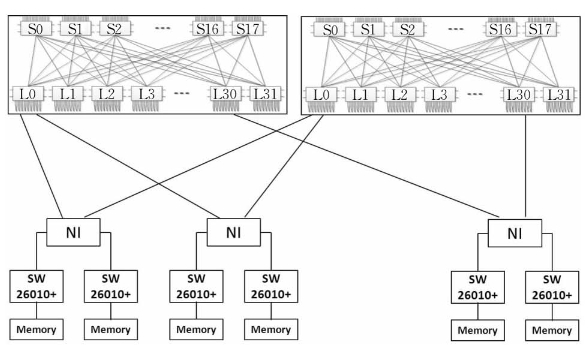
\includegraphics[scale=0.3]{神威E级.png}
	\caption{Caption}
	\label{fig:E}
\end{figure}

\section{国内外超算对比}
\subsection{国外超算概览——Frontier和富岳}
Frontier 是美国第一个性能超过 1 Exaflop/s的系统，位于美国田纳西州橡树岭国家实验室（ORNL），它使用了 8,699,904 个核心，目前实现了 1.194 Exaflop/s的性能。它基于 HPE Cray EX 架构，结合了第三代 AMD EPYC CPU（针对 HPC 和 AI 优化）、AMD Instinct 250X 加速器以及 Slingshot-11 互连。

Frontier计算系统安装在74个独立的机柜中，包括9400个CPU（标准计算机处理器）和37000个GPU，这些GPU可用于呈现3D图形，也可用于其他一系列任务。该机器共有8730112个内核，能够执行并行计算任务。\cite{7}

富岳采用ARM架构处理器，成为全球首台基于此架构进入TOP500排行榜的超级计算机。相较于其前身“京”（K computer），富岳在执行性能上实现了显著提升，最高可达“京”的100倍。这得益于大规模部署富士通定制的A64FX处理器，该处理器专为高性能计算优化，支持高带宽内存和可扩展性。

富岳的核心硬件组件是富士通定制的A64FX处理器，基于ARMv8.2-A架构，专为高性能计算优化。每个处理器拥有48个计算核心，支持SVE（Scalable Vector Extensions）指令集，能够处理长达512位的向量操作，极大地提升了浮点运算能力和并行处理效率。\cite{8}
这种设计使得富岳在科学计算、大数据分析等领域具有出色的表现。富岳由约400台机柜组成，每台机柜包含多个计算节点。这些节点通过高效互联网络连接，形成一个庞大而高度协同的计算集群。系统整体设计注重空间利用率、散热效率和维护便捷性，展现了高度工程化的硬件集成水平。

\subsection{国内外超算对比}
\subsubsection{性能对比}
美国Frontier超算（2022年）作为全球首台E级（百亿亿次）超算，峰值算力达1.4 EFLOPS（每秒百亿亿次浮点运算），在传统科学计算领域仍保持领先地位。其采用AMD EPYC CPU与Instinct GPU的异构架构，能效比显著优于中国神威·太湖之光。然而，中国在数据密集型应用领域展现出独特优势。2024年11月，“天河”超算以22301.67MTEPS/W的能效比登顶Graph500小数据图计算榜单，同时在GreenGraph500大数据能效榜单蝉联冠军，凸显其在图计算这一新兴领域的全球领先地位。\cite{9}
日本富岳（2020年）以442PFLOPS的算力曾登顶全球，其Arm架构A64FX芯片更侧重能效平衡（15.6 GFlops/W），在复杂网络分析等场景中表现突出，例如COVID-19病毒飞沫传播模拟。可见，中国超算在特定领域已实现局部超越，但整体能效与制程工艺仍存差距。

\subsubsection{技术路线博弈}
美国超算以x86+GPU的通用架构为主导，依托成熟的CUDA生态与商业芯片供应链快速迭代。例如，2025年即将部署的Aurora超算采用Intel Xeon Max CPU与Ponte Vecchio GPU，主打AI与科学计算的深度融合，但其核心硬件仍依赖全球化分工。日本则选择Arm架构的差异化路径，富岳通过定制化A64FX芯片实现高能效，但其软件生态适配成本较高，限制了应用扩展。中国则坚持“自主芯片+异构众核”路线，以神威系列申威处理器为例，单芯片集成260核心，通过片上网络优化通信效率，实现全链条国产化。然而，国产软硬件生态的短板仍制约发展。

\section{我国超算未来展望}
中国超算未来的发展需在技术、生态、应用三个维度实现突破，同时应对国际竞争与能效挑战。

AI与超算的深度结合：国外超算（如Frontier）已支持大规模AI训练，如美国橡树岭国家实验室利用Frontier训练生成式模型。中国“天河+AI”平台虽已部署，但应用场景仍以传统科学计算为主。混合精度计算和存算一体架构都可以是我们的突破方向。

量子-经典混合计算：量子计算可解决传统超算难以处理的组合优化问题（如材料模拟、密码破解），这是超算突破和创新的机遇。美国IBM已推出Qiskit Runtime量子-经典混合编程框架，我国需加速量子算法与超算的接口标准化。不过需要注意，量子硬件成熟度低，短期内难以替代经典超算，要避免资源过度倾斜。

绿色化转型是另一关键方向。技术路径一方面在于液冷与浸没式冷却，例如曙光E级超算已采用全浸没式液冷，功耗降低40\%。神威·太湖之光通过三维立体液冷系统将PUE值压至1.04，较传统风冷节能70\%。另一路径在于RISC-V架构探索，开源指令集可定制化优化能效。

中国超算历经四十余年发展，从银河系列到神威、天河系列，已实现从依赖进口到全技术链自主化的跨越。当前，我国在异构众核架构设计和绿色化等领域形成特色，但在芯片研发、软件生态及能效比上仍需进步。中国超算的未来不仅是算力的竞争，更是生态与治理能力的全面较量。唯有坚持“自主创新+开放合作”的双轨战略，方能在全球科技博弈中立于不败之地。


\newpage
\bibliographystyle{plain}
\bibliography{reference.bib} 

\end{document}